\documentclass[11pt, a4paper]{article}

\usepackage{amsmath}
\usepackage{amsfonts} %Matheschriften
\usepackage{amssymb} %Mathesymbole
%\usepackage{mathptmx} % Einstellung für Schriften und Sonderzeichen in mathematischen Umgebungen
                        % ändert SChriftfont
\usepackage{wasysym} % Stellt diverse Sonderzeichen bereit
\usepackage{siunitx}
\usepackage{float}
\usepackage{microtype}
\usepackage{graphicx}
\usepackage{hyperref}
\usepackage{xcolor}
\usepackage[section]{placeins}
% allows for temporary adjustment of side margins
\usepackage{changepage}
\usepackage{rotating}
\usepackage{tikz}
\usetikzlibrary{arrows,calc,decorations.markings}


\usepackage[ngerman]{babel}
\addto\captionsngerman{%
 \renewcommand{\abstractname}{Einleitung}}

\title{Versuch 4: Optik}
\author{Team 4-11: Jascha Fricker, Benedict Brouwer}
\date{17.3.2023}

\begin{document}

    \pgfarrowsdeclarecombine{|<}{>|}{latex}{latex}{|}{|}
    \def\Dimline[#1][#2][#3]{
        \begin{scope}[>=latex] % redef arrow for dimension lines
            \draw let \p1=#1, \p2=#2, \n0={veclen(\x2-\x1,\y2-\y1)} in [|<->|,
            decoration={markings, % switch on markings
                    mark=at position 0.5 with {\node[#3] at (0,0) {\DimScale{\n0}};},
            },
            postaction=decorate] #1 -- #2 ;
        \end{scope}
    }

    \def\DimScale#1{\pgfmathparse{round(#1/28.4*10.0)/10.0}\pgfmathresult cm}

    \maketitle

    \tableofcontents

    \newpage

    \section{Einleitung}
    In der Physik spielen Linsen in optischen Versuchsuafbauten eine sehr wichtige Rolle. In diesem Versuch soll es darum gehen, verschiedene 
    Methoden auszuprobieren um den Brechungsindex und Hauptebenenabstand verschiedener Lisnen bzw Linsensysteme zu messen.

    \section{Allgemeine Theorie}
    \FloatBarrier
    In der Physik spielen Linsen in optischen Versuchsuafbauten eine sehr wichtige Rolle. In diesem Versuch soll es darum gehen, verschiedene 
    Methoden auszuprobieren um den Brechungsindex und Hauptebenenabstand verschiedener Lisnen bzw Linsensysteme zu messen.
    \subsection{Autokollimation}
    Wie in Abbildung \ref{fig:autoKollAbb} zu sehen ist, wird die zu untersuchende Linse zwischen Blende und Spiegel gestellt. Nun wird der Abstande $l$ zwischen 
    Linse und Blende so eingestellt, dass auf der Blende welche gleichzeitig als Schirm dient ein Scharfes Bild entsteht. Dieser Vorgang wird wiederholt mit der um $180^\circ$ gedrehten Linse und der Abstand $k$ gemessen.
    Aus diesen Daten lassen Sich Brechungsindex und Hauptebenenabstand wie folgt berechnen:

    \begin{align}
    f' = \frac{k+l-h}{2} \label{eq:autokollBrech}\\
    h = k + l - 2 \cdot f' \label{eq:autokollHaupt}
    \end{align}

    \begin{figure}
        \centering
        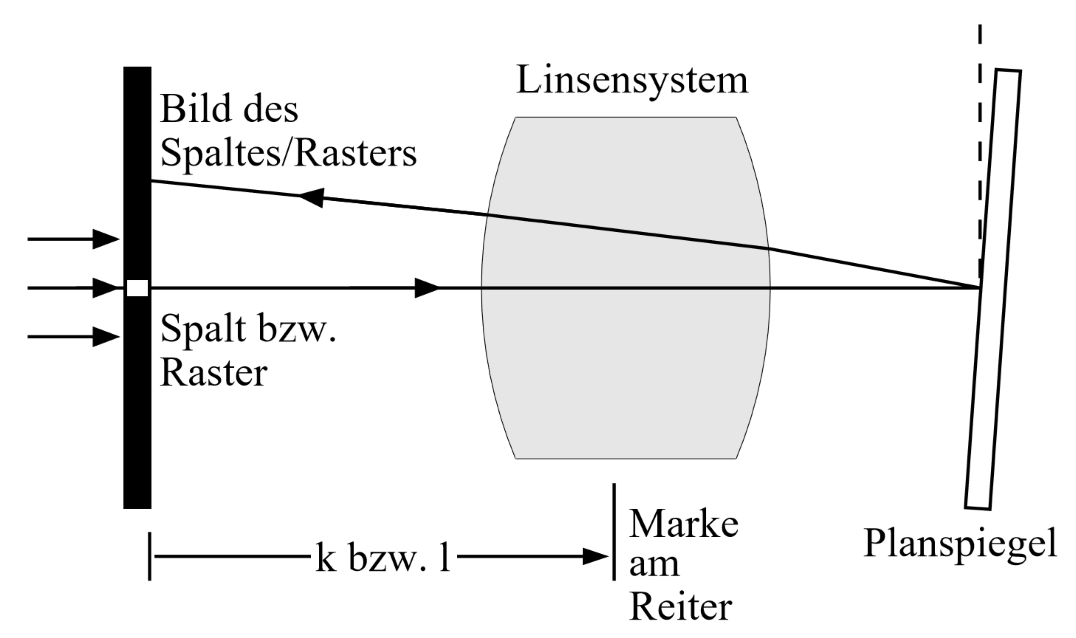
\includegraphics[width=0.8\textwidth]{Autokollimation_abb.png}
        \caption{Versuchsaufbau zum Autokollimationsverfahren \cite{OPA}}   % Quelle Fehlt
        \label{fig:autoKollAbb}
    \end{figure}

    \subsection{Besselmethode}
    Bei der Besselmethode wird die zu untersuchende Linse zwischen Blende und Schirm wie in Abbildung \ref{fig:BesselAbb} veranschaulicht gestellt.
    Es gibt nun zwei Positionen, bei denen ein scharrfes Bild auf dem Schirm entsteht. Aus der Differenz dieser Positionen und dem Abstand von Blende und Linse folgt nun für den Brechungsindex und den Hauptebenenabstand:
    \begin{align}
        f' = \frac{1}{4} \cdot [(e-h)-\frac{d^2}{e-h}] \label{eq:besselBrech1}\\
        f = \frac{1}{4} \cdot [\frac{d^2}{e-h}-(e-h)] \label{eq:besselBrech2}
    \end{align}
    

    \begin{figure}
        \centering
        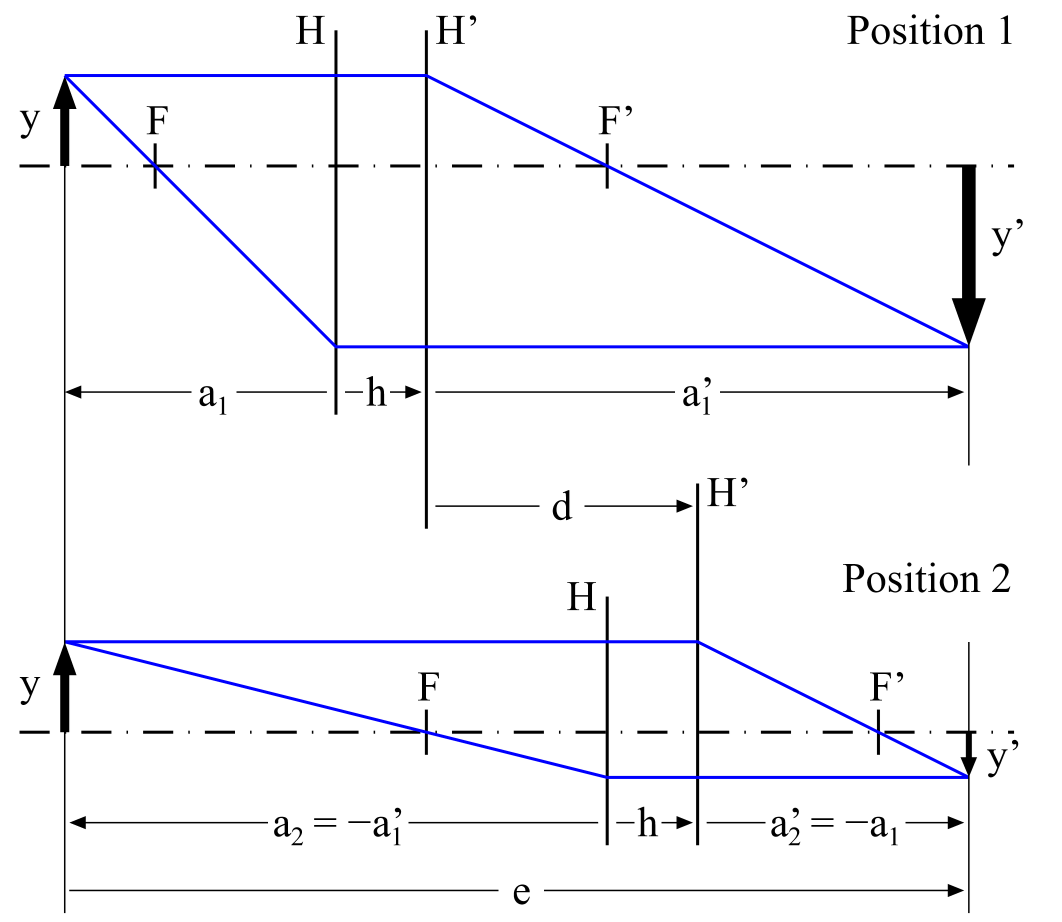
\includegraphics[width=0.8\textwidth]{Bessel_Abb.png}
        \caption{schematischer Versuchsaufbau der Besselmethode \cite{OPA}}   % Quelle Fehlt
        \label{fig:BesselAbb}
    \end{figure}

    \subsection{Abbemethode}

    Bei der Messmethode nach Abbe werden die position der Hauptachsen und Brennweiten der Linsensysteme gemessen. 

    \subsection{Dünne Linsen speziefisch}
    Bei Dünnen Linsen kann der Abstand $h = 0$ zwischen den beiden Haupachsen vernachlässigt werden.
    
    \paragraph{Autokollimationsmethode}
    Bei Autokollimationsmethode wird der Aufbau so aufgebaut, dass das Bild und Objekt auf gleicher Position sind. Auf der anderen Seite der Linse reflektiert ein Spiegel die parallelen Strahlen. Wenn das Bild scharf ist, ist die Brennweite
    \begin{align}
        f = \frac{k + l - h}{2}  = d \label{eq:auto}
    \end{align}
    bei dünnen Linsen $h=0$ genau der Abstand $d = k = l$ zwischen Objekt/Bild und Linse.

    \paragraph{Besselmethode}
    Bei der Besselmethode kann die Brennweite
    \begin{align}
        f = \frac{1}{4} \left( e - \frac{d^2}{e} \right) = \frac{1}{4} \left( e - \frac{\left(a_2 - a_1\right)^2}{e} \right) \label{eq:bessel}
    \end{align}
    durch die zwei Positionen der Linse $a_1$ und $a_2$ und den Abstand Objekt-Schirm $e$ bestimmt werden.
    
    \subsection{Optisches System}

    Für die Gesamtbrennweite und Hauptebenen eines Optischen Systems gilt
    \begin{align}
        f &= \frac{f_1' \cdot f_2'}{t - f_1' - f_2'} \label{eq:brenn}\\ 
        \begin{split} \label{eq:ebene}
           z &= \frac{f_1 \cdot t}{t - f_1' - f_2'}  \\
           z' &= \frac{f_2 \cdot t}{t - f_1' - f_2'} \\
           h &= \frac{t}{t - f_1' - f_2'}
        \end{split}
    \end{align}

    \paragraph{Bessel- und Autokollimationsmethode}
    Bei dicken Linsen kann durch zusammenführen der Besselmethode und Autokollimationsmethode die Brennweite $f'$ und der Hauptebenenabstand $h$
    
    \begin{align} \begin{split} \label{eq:dicke}
        f' &= \frac{1}{2} \sqrt{(e-k-l)^2 - d^2} \\
        h &= k + l - \sqrt{(e-k-l)^2 - d^2} \end{split}
    \end{align}
        
    bestimmt werden. Dabei ist $d = a_2 - a_1$ die Distanz zwischen den beiden Positionen der Linse, $e$ der Abstand zwischen Objekt und Schirm, $k$ der Abstand zwischen Linse und Objekt/Bild und $l$ der Abstand zwischen Objekt/Bild bei umgedrehten Linsensystem.

    \paragraph{Messmethode nach Abbe}
    Es gelten die zwei Beziehungen
    \begin{align}
        g &= f \cdot \left(1 - \frac{1}{\beta}\right) + h_1 \label{eq:dicke1} \\
        g' &= f' \cdot (1 - \beta) + h_2 \label{eq:dicke2} \\
        \text{mit} \ \ \beta &= \frac{y'}{y}
    \end{align}
    Durch fitten an die Daten für den Abstand zum Objekt $g$ bzw zum Bild $g'$ kann die Brennweite $f$ bzw $f'$ und der Hauptebenenabstand $h_1$ und $h_2$ bestimmt werden.


    \section{Ergebnisse}
    \subsection{Aufgabe 1}
    Als erstes wurden alle Linsen angeschaut. Durch beobachten des Millimeterpapiers durch die Linsen konnte zwischen einem vergrößernden Effekt (Konvexe Linse) und einem verkleinerndem Effekt (Konkave Linse) unterschieden werden. Nur die Linse E konnte als Streulise identifiziert werden, alle anderen Linsen waren als Sammellisen zu erkennen.

    \subsection{Einzellinsen}
    Die Ergebnisse der Autokollimationsmethode und der Besselmethode sowie der gewichtete Mittelwert der beiden Methoden wurden mit den Formel (\ref{eq:auto}) und (\ref{eq:bessel}) sind in der Tabelle \ref{tab:ergebnisse} dargestellt.

    \begin{table}[h]
        \centering
        \begin{tabular}{c|c|c}
            Methode & Brennweite B & Brennweite G \\ \hline
            Autokollimation & $10,04(5) \si{\centi\metre}$ & $7,49(7) \si{\centi\metre}$ \\ \hline
            Bessel & $9,97(8) \si{\centi\metre}$ & $7,488(35) \si{\centi\metre}$ \\ \hline
            Mittelwert & $10.02(4) \si{\centi\metre}$ & $7.492(31) \si{\centi\metre}$
        \end{tabular}
        \caption{Brennweiten der Linsen B und G}
        \label{tab:ergebnisse}
    \end{table}
    Der Fehler der Länge wurde mit Tabelle 5 des ABW-Skripts \cite{ABW} berechnet und durch den gewichteten Mittelwert fortgepflanzt.

    \subsection{Linsensystem}
    Wir haben das Linsensystem E-G mit $30$ mm Abstand für unsere Messungen benutzt. Wobei die Linse E die erste im Strahlengang ist. Dies ist genau anders herum wie in der Aufgabenstellung.

    \paragraph{Autokollimation- und Besselmethode}
    Mit Gleichung \ref{eq:dicke} konnte aus den Messwerten der beiden Methoden die Brennweite und der Hauptebenenabstand
    \begin{align}
        f' &= 13,10(20) \si{\centi\metre} \\
        h &= 0,3(6) \si{\centi\metre}
    \end{align}
    bestimmt werden. Der Fehler der Länge wurde mit Tabelle 5 des ABW-Skripts \cite{ABW} berechnet und der gewichtete Mittelwert wurde genutzt.

    \paragraph{Messmethode nach Abbe}
    Um die Brennweiten und Hauptebenenabstände zu bestimmen,
    \begin{align}
        f &= 14,22(34) \si{\centi\metre} \\
        f' &= -12,74(19) \si{\centi\metre} \\
        h_1 &= 6,81(73) \si{\centi\metre} \\
        h_2 &= 6.82(87) \si{\centi\metre}
    \end{align}
    
    wurden die Messwerte für den Abstand zum Objekt $g$ und zum Bild $g'$ mit den Formeln (\ref{eq:dicke1}) und (\ref{eq:dicke2}) gefittet. Die Fits sind in \ref{fig:fit1} und \ref{fig:fit2} dargestellt. Alle Angaben sind relativ zur Linse E. Die Angaben stimmen in etwa mit den Ergebnissen der Autokollimationsmethode und der Besselmethode überein, die Hauptebenen haben aber eine sehr große Unsicherheit.

    \begin{figure}[h]
        \centering
        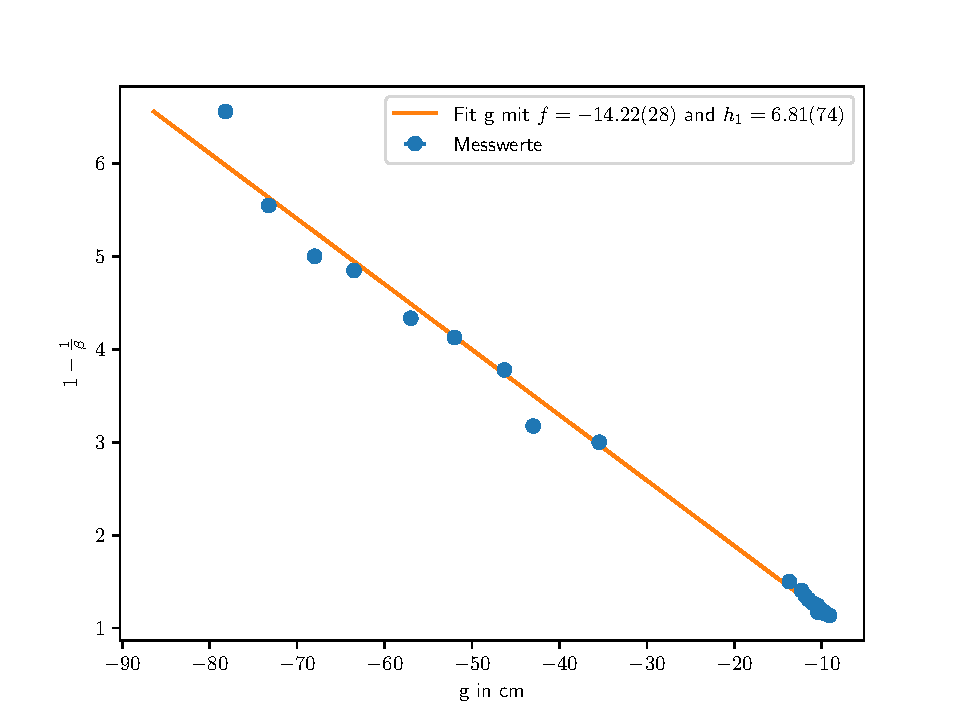
\includegraphics[width=0.8\textwidth]{g.pdf}
        \caption{Fit der Messwerte für den Abstand zum Objekt}
        \label{fig:fit1}
    \end{figure}

    \begin{figure}[h]
        \centering
        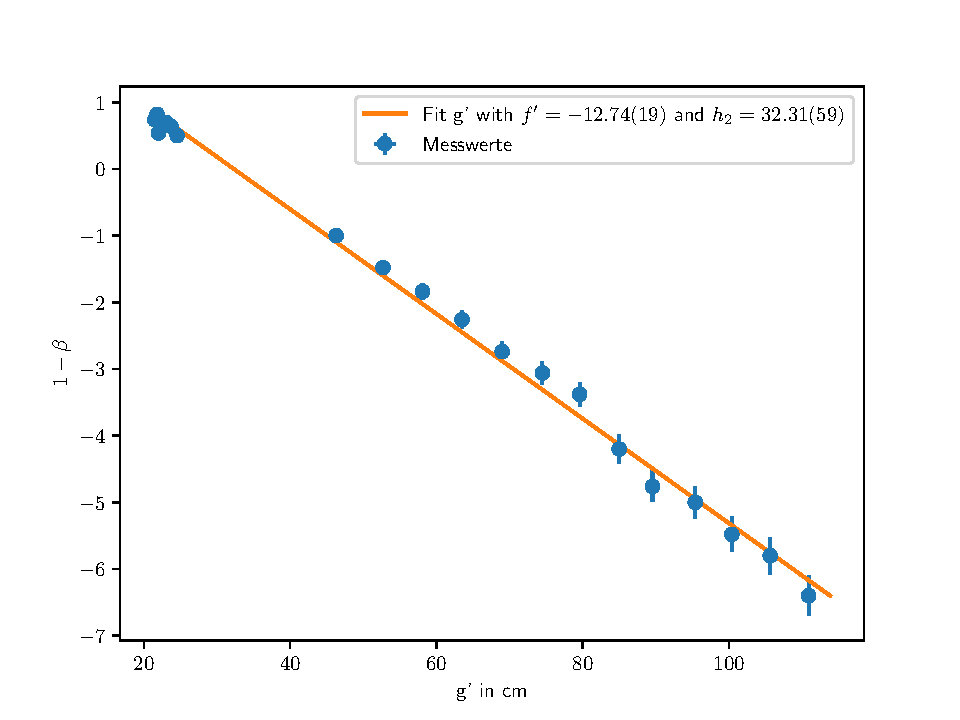
\includegraphics[width=0.8\textwidth]{g_prime.pdf}
        \caption{Fit der Messwerte für den Abstand zum Bild}
        \label{fig:fit2}
    \end{figure}

    % Bild des Aufbaus


    \begin{figure}[h]
        \centering
        \begin{tikzpicture}[scale=0.3]
            % Define lens properties
            \def\lensRadius{10}
            \def\lensHeight{12}
            \def\lensWidth{1}
            \def\focalLengthOne{-5} % concave lens
            \def\focalLengthTwo{5} % convex lens
            \def\startAngle{asin(\lensHeight/\lensRadius)}
            \pgfmathsetmacro{\lensRadius}{50}
            \pgfmathsetmacro{\lensHeight}{10}
            \pgfmathsetmacro{\startAngle}{asin(\lensHeight/\lensRadius)}


            % Draw lenses
            \draw [fill=blue!15]  (3,\lensHeight)
            arc[start angle=180-\startAngle,delta angle=2*\startAngle,radius=\lensRadius]
            arc[start angle=-\startAngle,delta angle=2*\startAngle,radius=\lensRadius]
             -- cycle; % to get a better line end
            \draw [fill=blue!15] (\lensWidth,\lensHeight)
            arc[start angle=180-\startAngle,delta angle=2*\startAngle,radius=\lensRadius] -- (-\lensWidth, -\lensHeight)
            arc[start angle=-\startAngle,delta angle=2*\startAngle,radius=\lensRadius]
             -- cycle; % to get a better line end
            % Draw principal planes
            \draw [dashed] (6.806, -1*\lensHeight) -- (6.806, 1*\lensHeight);
            \draw [dashed] (6.827, -1*\lensHeight) -- (6.827, 1*\lensHeight);

            % Draw focal points
            \filldraw (- 14.217 + 6.806,0) circle (4pt);
            \filldraw (12.741 + 6.827 ,0) circle (4pt);

            % Label lenses
            \node at (0,-14) (E) {E};
            \node at (3,-14) (G) {G};

            % Label principal planes and focal points
            \node at (6.806,-14) (P1) {};
            \node at (6.806,-13) {$H_1$};
            \node at (- 14.217 + 6.806,-14) (F1) {$F_1$};
            \node at (6.827,-14) (P2) {$H_2$};
            \node at (12.741 + 6.827 ,-14) (F2) {$F_2$};

            \Dimline[($(E)+(0,-2)$)][($(G)+(0,-2)$)][below];
            \Dimline[($(P2)+(0, 3)$)][($(F2)+(0, 3)$)][above];
            \Dimline[($(G)+(0,-2)$)][($(P2)+(0,-2)$)][above];
            \Dimline[($(P1)+(0, 2)$)][($(F1)+(0, 2)$)][above];
            \Dimline[($(E)+(0,-4)$)][($(P1)+(0,-4)$)][below];

            % Draw optical axis
            \draw [->](-10,0)--(25,0);

            % Label optical axis
            %\node at(30,-3){Optical Axis};

        \end{tikzpicture}
        \caption{Linsensystem E-G 30mm}
        \label{fig:aufbau}
    \end{figure}


    \subsubsection{Berechnung der Brennweiten und Hauptebenen}
    \paragraph{Brennweite}
    Durch umstellen der Gleichung (\ref{eq:brenn}) nach $f_E$ kann die Brennweite der ersten Linse E bei durch Aufgaben 2 und 3 gegebener Brennweite $f_G = 7.492(31) \si{\centi\metre}$ und $f' = - 13,10(20) \si{\centi\metre}$ berechnet werden. Der Abstand $t = 3 \si{\centi\metre}$ ist auch gegeben.

    \begin{align}
        f_E = \frac{f' \left(t - f'\right)}{f' - f_G} = 10.24(20) \si{\centi\metre}
    \end{align}

    Diese Wert für $f_E$ stimmt sehr gut mit der Vorgabe überein, hat aber nur eine kleine Unsicherheit.

    \paragraph{Hauptebenen}
    Die Abstand der Haubtebenen von den jeweiligen Linsen $z$ und $z'$ sowie der relative Abstand $h$ kann durch Gleichungen (\ref{eq:ebene}) berechnet werden. Dabei gilt $f_1' = -f_1 = f_E' = -10 \si{\centi\metre}$ und $f_2' = f_G' = 7.492(31) \si{\centi\metre}$.
    \begin{align}
        z &= \frac{f_1 \cdot t}{t - f_1' - f_2'} = 5.447(89) \si{\centi\metre} \\
        z' &= \frac{f_2 \cdot t}{t - f_1' - f_2'} = 4.081(74) \si{\centi\metre} \\
        h &= \frac{t}{t - f_1' - f_2'} = 0.5447(89) \si{\centi\metre}
    \end{align}
    Der Wert von $h$ rechnerisch und graphisch liegen innerhalb der Unsicherheit, die Werte von $z$ und $z'$ sind jedoch nicht innerhalb der Unsicherheiten von $h_1$ und $h_2 - 3 \si{\centi\metre}$. Dies kann an einer Ungenauen bestimmung durch die Abbe Methode liegen.

    \paragraph{Simulation}
    In Abbildung \ref{fig:fit2} ist die Simulation des Strahlenverlaufs für die Optik G-E veranschaulicht. Da unser Aufbau genau andersherum ist, muss die Optik G-E umgedreht werden. Die Simulation zeigt, dass die Lage der entscheidenden Punkte qualitativ mit den von uns bestimmten Werten übereinstimmen. Die Hauptebenen sind in der Simulation etwas weiter auseinander als bei uns. Dies kann an der Ungenauigkeit der Abbe Methode liegen.

    \begin{figure}[h]
        \centering
        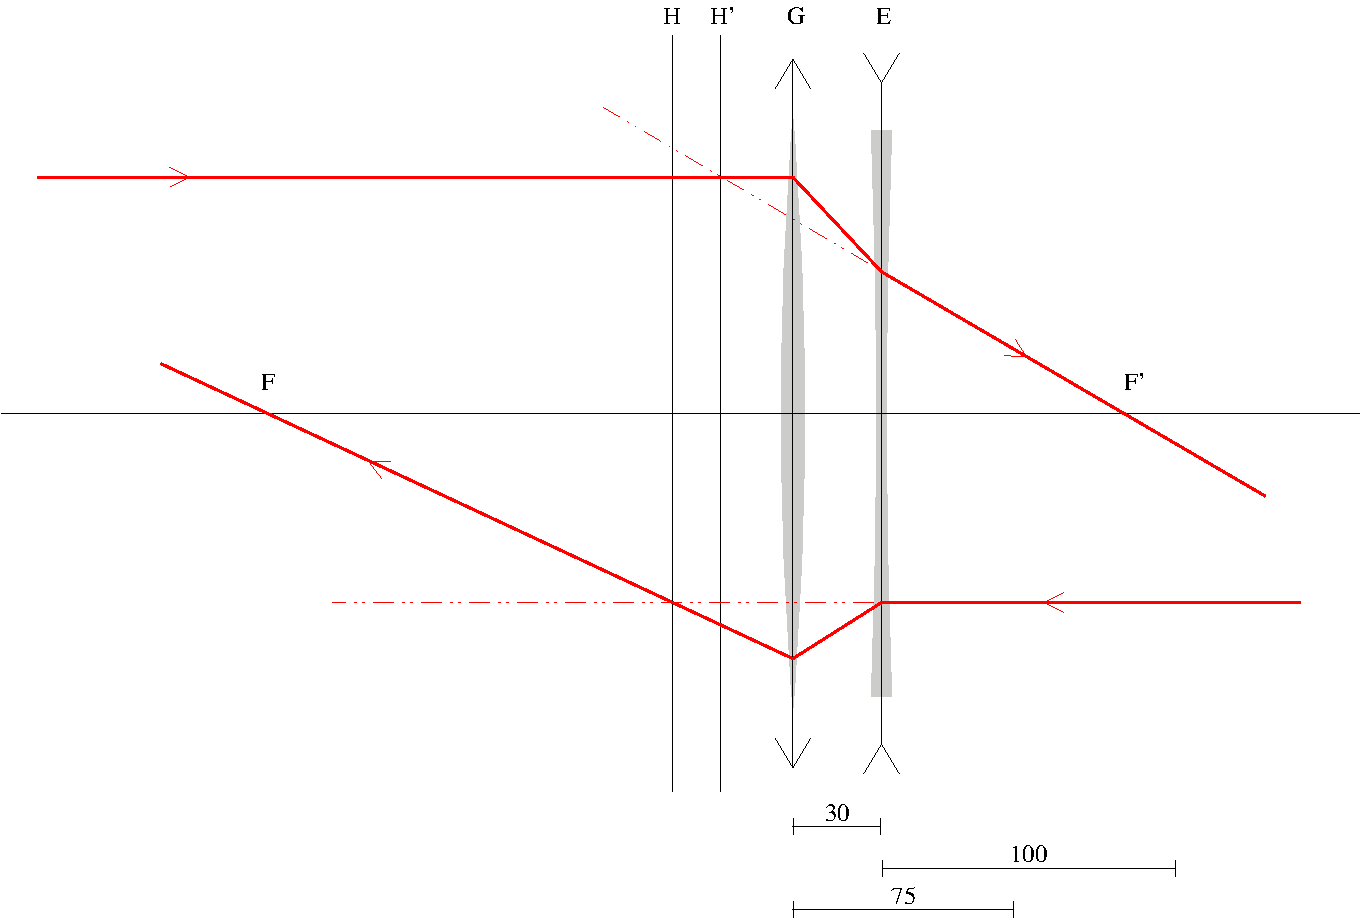
\includegraphics[width=0.8\textwidth]{G-E-30.pdf}
        \caption{Simulation des Strahlenverlaufs für die Optik G-E}
        \label{fig:fit2}
    \end{figure}

    \section{Fragen}
    \begin{itemize}
        \item Beim Bessel-Verfahren gibt es zwei Positionen des Linsensystems, an denen eine scharfe Abbildung möglich ist. Aufgrund der Umkehrbarkeit des Strahlengangs entsprechen die objektseitigen Größen im ersten Fall gerade den bildseitigen Größen im Zweiten. Das heißt die Abbildungsmaßstäbe sind genau die Kehrwerte voneinander.
        \item In einem Projektionsapparat wird die Lampe hinter einem Hohlspiegel angeordnet. Der Kondensor ist eine Linsenkombination, die wie eine Sammellinse wirkt und so angeordnet ist, dass das Dia gut ausgeleuchtet ist und das gesamte vom Dia ausgehende Licht ins Objektiv trifft. Auf diese Weise entsteht ein vollständiges, höhen- und seitenverkehrtes, vergrößertes Bild vom Original auf der Leinwand. Der Schemtaische Aufbau wird in Abbildung \ref{fig:projektionsapparat} dargestellt.
        \item Wenn sich das Objekt in einem Abstand von a = 0,5 · f von der objektseitigen Hauptebene einer Sammellinse befindet, dann ist a < f. In diesem Fall entsteht ein virtuelles Bild, das nicht auf dem Kopf stehen und größer als der Gegenstand ist. Der Abbildungsmaßstab ist 2 und die Position $a'= f$ ist genau der gegenstandsseitige Brennpunkt.
        \item Die Gesamtbrennweite eines Systems zweier Sammellinsen gleicher Brennweite kann durch die Verwendung der Linsengleichung berechnet werden. Die Linsengleichung lautet: $\frac{1}{f} = \frac{1}{f_1} + \frac{1}{f_2} - \frac{t}{f_1 f_2}$, wobei $f$ die Gesamtbrennweite des Systems ist, $f_1$ und $f_2$ die Brennweiten der beiden Linsen und $t$ der Abstand zwischen den beiden Linsen.
        In diesem Fall haben beide Linsen die gleiche Brennweite ($f_1 = f_2$), so dass sich die Gleichung vereinfacht zu: $\frac{1}{f} = \frac{2}{f_1} - \frac{t}{f^2_1}$. 
    \end{itemize}

    \begin{figure}[h]
        \centering
        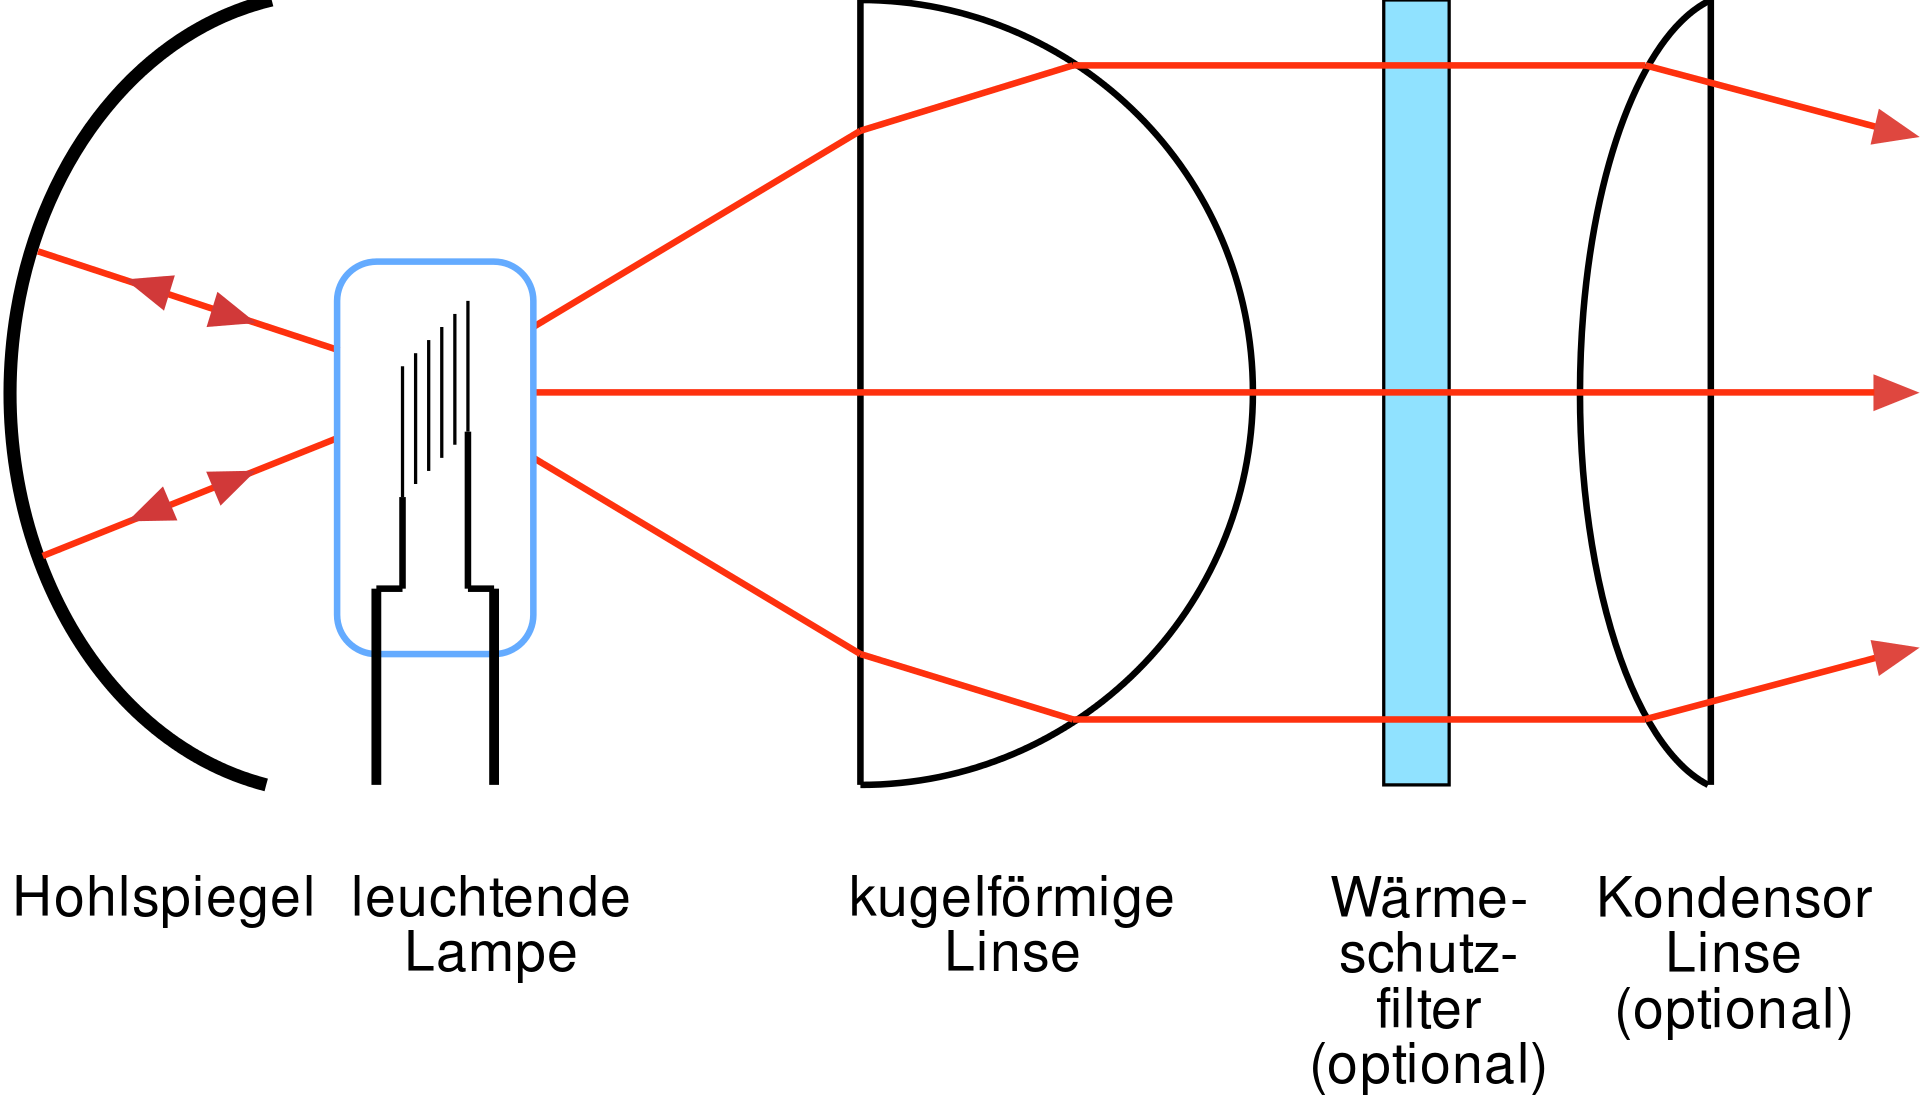
\includegraphics[width=0.8\textwidth]{Condensor-1-de.svg.png}
        \caption{Schematischer Aufbau eines Projektionsapparates nach \cite{projektionsapparat}}
        \label{fig:projektionsapparat}
    \end{figure}




    \section{Diskussion}

    \bibliographystyle{plain}
    \bibliography{literature}

\end{document}